\section{Einbindung in OSSIM}

\label{sec_impl_integration_into_ossim}

%- Vorgehen
%
%- Nur für Syslog, keine anderen Fomate betrachtet
%
%- Syslog-Nachrichten werden entgegengenommen, geparst und Config-basiert einzelne Datenfelder bearbeitet (basierend auf RegEx)
%
%- Konfigurationsdateien für Datenquellen (leichte Erweiterbarkeit, auch im Bezug auf neue Datenquellen, ...) mit Beispiel
%
%- Plugins (leichte Erweiterbarkeit, ...)

Wie in Abschnitt \ref{sec_state_siem} beschrieben, erlaubt OSSIM eine verteilte Installation am Empfang von Logdaten beteiligter Komponenten durch die Einführung optionaler Sensoren, die den Empfang und das Parsen von Logdaten übernehmen. Dadurch bieten sich gegenüber den in Abschnitt \ref{sec_over_dataflow_siem} beschriebenen Möglichkeiten zum Eingriff in den Datenfluss eines SIEM-Systems zwei weitere OSSIM-spezifische Möglichkeiten, die folgend als mögliche Alternativen beschrieben werden. Eine Übersicht über den entstehenden Datenfluss bietet Abbildung \ref{fig:ossim_data_access_point}. Die Ziffern beschreiben die Stelle des Eingriffs, wie in der Abbildung gekennzeichnet:

\begin{figure}[]
    \centering
        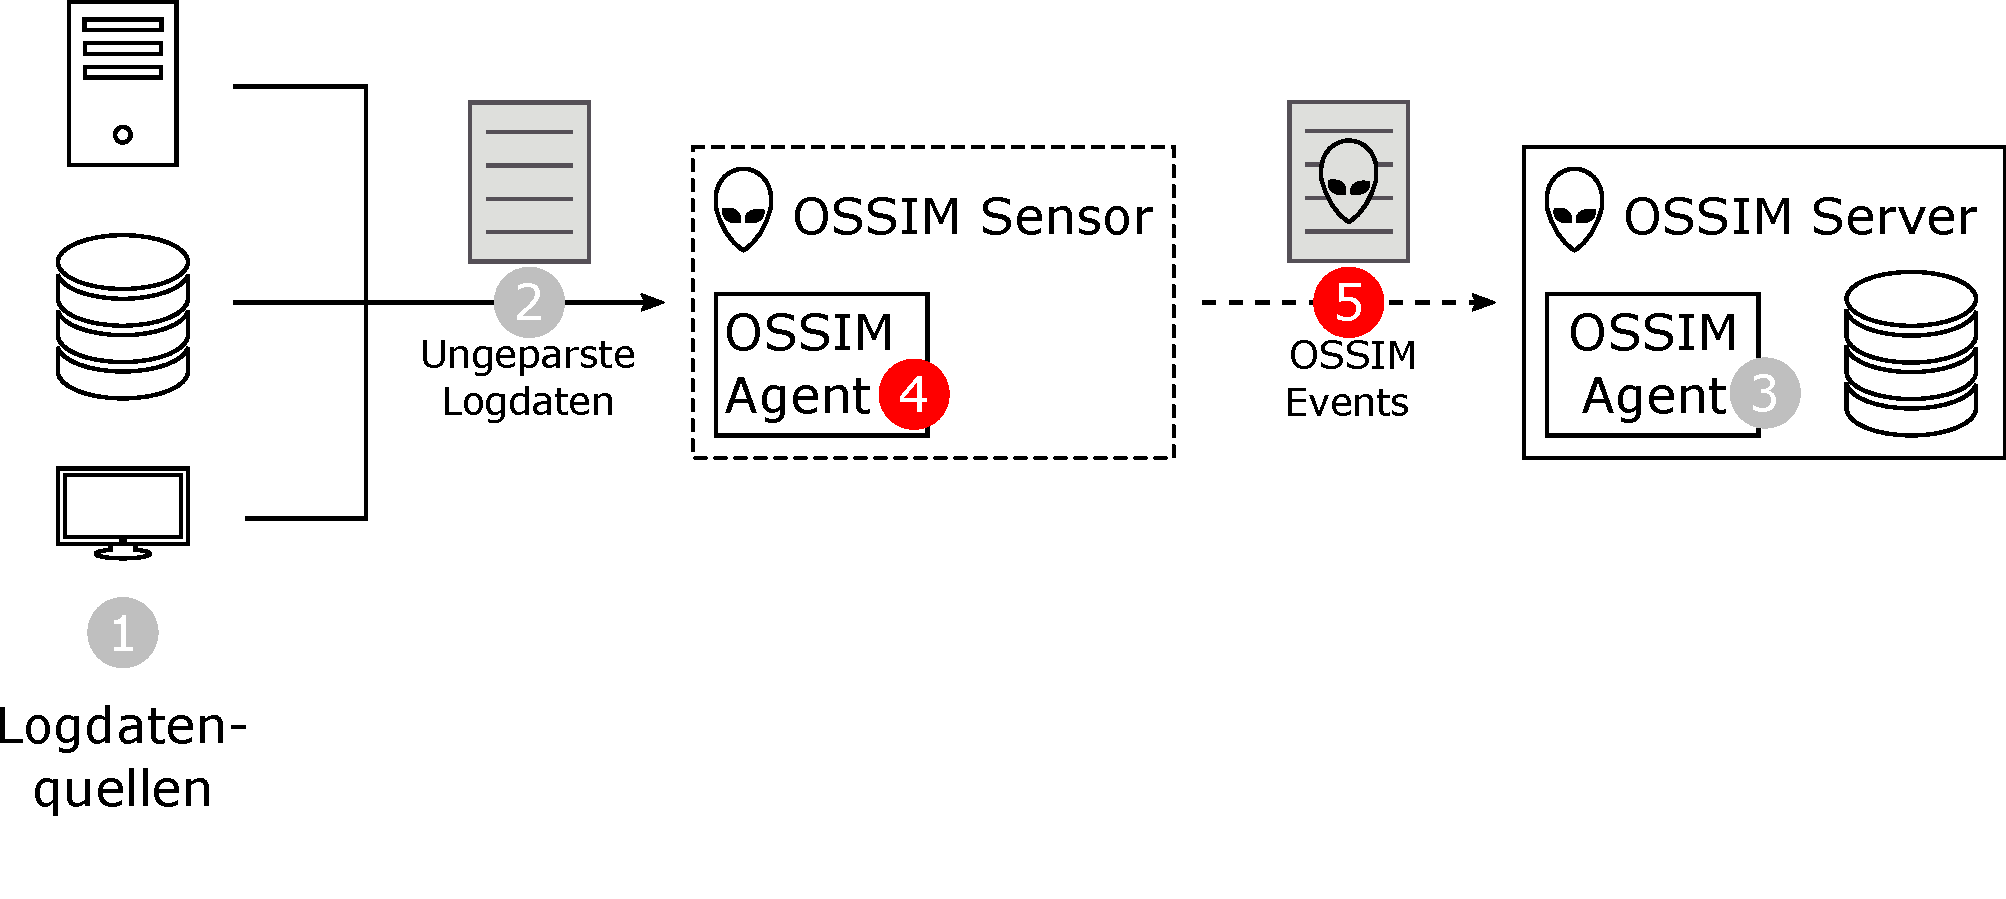
\includegraphics[width=0.9\textwidth]{dia/ossim_data_access_point.pdf}
    \caption{Mögliche Eingriffspunkte in den OSSIM-Datenfluss.}
    \label{fig:ossim_data_access_point}
\end{figure}

\begin{enumerate}
\setcounter{enumi}{3}

\item \textbf{Patchen des OSSIM-Sensor-Agents}\\
  Bei dieser Lösung müsste der OSSIM-Agent des Sensors so verändert werden, dass vor dem Senden der Events an den Server die Pseudonymisierung stattfindet. Daten erreichen den OSSIM-Server nur pseudonymisiert und mehrfaches Parsen der Logdaten wird verhindert. Auf der anderen Seite erfordert diese Lösung einen Eingriff in die Funktionsweise von OSSIM, was beispielsweise bei Updates von OSSIM zu Problemen führen kann. Außerdem liegen die Daten zu Beginn in nicht-pseudonymisierter Form im Sensor vor -- ein Nachteil der bereits in Abschnitt \ref{sec_state_siem} ausführlich diskutiert wurde. Zusätzlich erfordert diese Lösung die verteilte Installation von OSSIM-Sensor und -Server, schließt also die All-In-One-Installation aus.
  
\item \textbf{Sensor-Server-Proxy}\\
  Hier wird ein Proxy zwischen Sensor und Server geschaltet, der bereits geparste Events pseudonymisiert und anschließend an den Server sendet. Dieser Ansatz würde mehrfaches Parsen verhindern und dafür sorgen, dass nur pseudonymisierte Logdaten den OSSIM-Server erreichen. Wie die vorhergehende Lösung würde er jedoch nur in der verteilten Installation funktionieren und zusätzlich in die Kommunikation zwischen Sensor und Server aktiv eingreifen, was im Hinblick auf die Nachrichtenintegrität\footnote{
    In der aktuellen Version von OSSIM werden Nachrichten unverschlüsselt und nicht signiert zwischen Sensor und Server versendet, aber zu hoffen ist, dass dieser Zustand sich in zukünftigen Versionen noch ändert.
  } und auch auf geändertes Verhalten nach Updates von OSSIM einen Nachteil darstellt.
\end{enumerate}

% Warum weiterhin Stelle 2?
% Beschränkung auf Syslog, Erweiterung um weitere Protokolle ähnlich
% Ansatz: Nimm syslog-Events entgegen, Verändere Felder abhängig von Config (su) mithilfe von PLugins (su), sende verändertes event weiter 
%

Die beiden weiteren Möglichkeiten leiden also unter denselben Nachteilen wie der Ansatz einer Veränderung des SIEM-Servers und sind zusätzlich nur bei der Nutzung von OSSIM einsatzbar.
Deshalb wurde sich für den zu entwickelnden Prototypen dazu entschieden, die bereits in Abschnitt \ref{sec_over_dataflow_siem} präferierte Lösung eines Proxys zwischen Datenquelle und SIEM-System umzusetzen.

Weiterhin wird sich auf den am häufigsten\footnote{
  Die in OSSIM bereits mitgelieferten Plugins bestätigen dies. Unter den Hunderten Plugins ist nur ein einziges, das einen anderen Mechanismus als das Syslog-Protokoll nutzt. Auch wenn beispielsweise Plugins, die eine Datenbankabfrage enthalten, immer dem Anwendungsfall angepasst und daher nicht in OSSIM inkludiert werden können, so unterstützt dies doch die Annahme des Syslog-Protokolls als am häufigsten genutzten Weg und damit als geeignet für den Fokus dieser Arbeit.
} genutzten Weg des Datenerhalts in OSSIM beschränkt: das Entgegennehmen der Daten über das Syslog-Protokoll (siehe Abschnitt \ref{sec_basics_siem_syslog}). Lösungen für weitere Wege (siehe Abschnitt \ref{subsec_state_siem_parsing}) sind bei Bedarf jedoch auf vergleichbarem Weg zu implementieren.

Der entwickelte Log-Proxy nimmt Logdaten über das Syslog-Protokoll entgegen. Verschiedene Datenquellen und Eventformate können mithilfe von Konfigurationsdateien angelegt werden, wie im nächsten Abschnitt beschrieben. Für einzelne Felder eines Logdatums können dabei Plugins angegeben werden, die die Behandlung des Feldes übernehmen. Der Proxy-Server kann durch einfach zu entwickelnde Plugins leicht um weitere Datenschutztechniken erweitert werden. Dies wird im übernächsten Abschnitt beschrieben. Nach der Behandlung eines Logdatums wird es anschließend über das Syslog-Protokoll an den OSSIM-Server oder -Sensor geschickt.

\subsection{Konfiguration von Datenquellen}
\label{sec_integration_in_ossim_datasource_config}

Die Behandlung von verschiedenen Datenquellen wird durch Konfigurationsdateien ermöglicht:

\begin{lstlisting}[morekeywords={general,active,pattern,group1,group2}]
[general]
active=True

[group1]
pattern=^(?P<time>\w+ *\d{1,2} \d{2}:\d{2}:\d{2}) (?P<device>[^:]+): Testing my device USER=(?P<user>.+)$
time=Substitute(substitute = 'somevalue_time')
device=Substitute(substitute = 'somevalue_device')
user=Pseudonymize()

[group2]
pattern=^(?P<test>.*)$
test=Pseudonymize()
\end{lstlisting}

Eine Konfigurationsdatei kann aus mehreren Bereichen bestehen. Der \texttt{general}-Bereich enthält allgemeine Angaben über das Plugin. Um unterschiedliche Lognachrichten eines Gerätes bündeln zu können, kann eine Konfigurationsdatei weiterhin mehrere Bereiche enthalten, die jeweils die Verarbeitung einer bestimmten Lognachricht beschreiben. Angegeben werden muss jeweils ein regulärer Audruck, der die Nachricht beschreibt und mehrere Gruppen (\texttt{(?P<name>...)}) enthalten kann. Für jede dieser Gruppen muss eine Angabe zu dem Plugin inklusive notwendiger Parameter gemacht werden, das die Gruppe verarbeiten soll. Durch diese Konfigurationsdateien können Nachrichten unbekannter Formate aus neuen Datenquellen leicht in das bestehende System eingebunden werden.

\subsection{Umsetzung von Datenschutztechniken durch Plugins}
\label{sec_integration_in_ossim_plugins}

Die Erweiterbarkeit um neue Datenschutztechniken wird durch leicht erweiterbare Plugins ermöglicht. Ein Plugin muss lediglich die Methode \texttt{handle\_data} implementieren, die die originalen Daten und alle in der Konfiguration angegebenen Parameter erhält. Ein einfaches Plugin, das die Daten durch einen in der Konfiguration angegebenen Wert ersetzt, könnte so aussehen:

\begin{lstlisting}[language=Python]
class Substitute(AbstractPlugin):

    def handle_data(self, data: str, **kwargs) -> str:
        if 'substitute' in kwargs:
            return kwargs['substitute']
        else:
            raise MissingSubstituteError
\end{lstlisting}